\documentclass{article}%
\usepackage[T1]{fontenc}%
\usepackage[utf8]{inputenc}%
\usepackage{lmodern}%
\usepackage{textcomp}%
\usepackage{lastpage}%
\usepackage[head=40pt,margin=0.5in,bottom=0.6in]{geometry}%
\usepackage{graphicx}%
%
\title{\textbf{Defensa de Requesens: Ministerio Público debe concluir su investigación}}%
\author{EL NACIONAL WEB}%
\date{28/09/2018}%
%
\begin{document}%
\normalsize%
\maketitle%
\textbf{URL: }%
http://www.el{-}nacional.com/noticias/presos{-}politicos/defensa{-}requesens{-}ministerio{-}publico{-}debe{-}concluir{-}investigacion\_253586\newline%
%
\textbf{Periodico: }%
EN, %
ID: %
253586, %
Seccion: %
Presos políticos\newline%
%
\textbf{Palabras Claves: }%
Diputados, Política, Presos políticos\newline%
%
\textbf{Derecho: }%
1.2%
, Otros Derechos: %
1.10%
, Sub Derechos: %
1.2.2, 1.10.1%
\newline%
%
\textbf{EP: }%
NO\newline%
\newline%
%
\textbf{\textit{Charity Flores denunció que el diputado a la Asamblea Nacional no ha tenido visistas de sus abogados desde su detención}}%
\newline%
\newline%
%
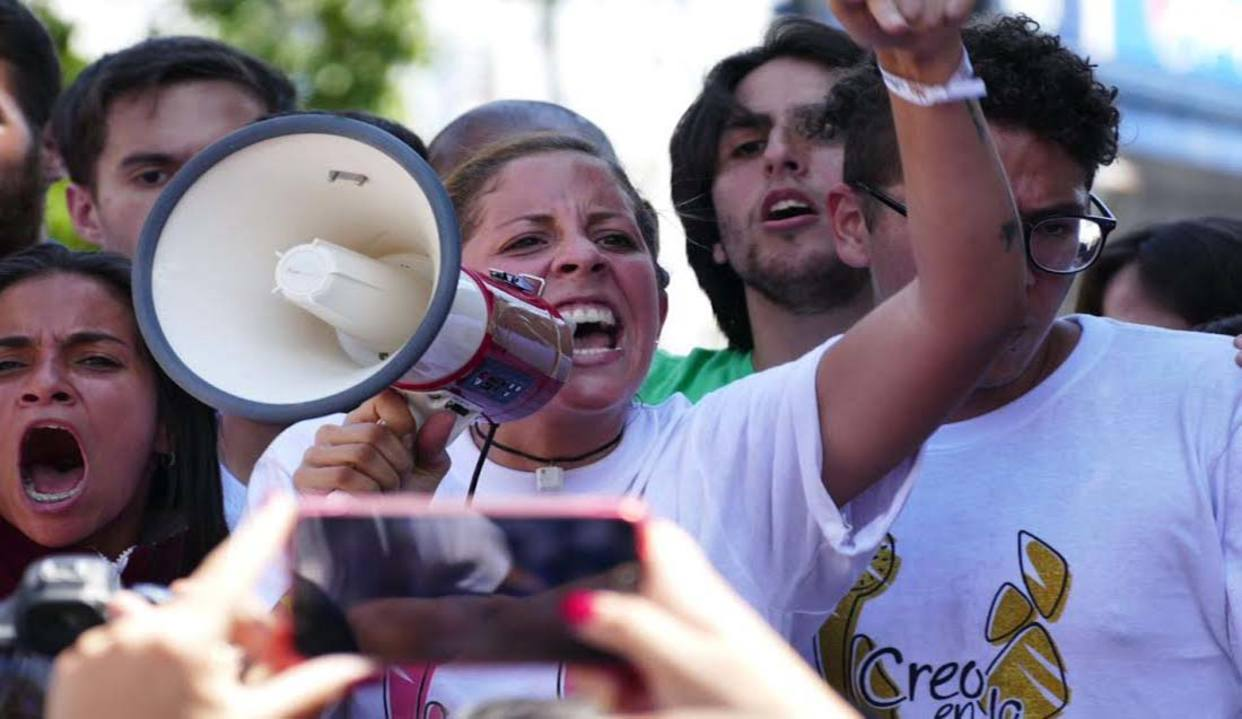
\includegraphics[width=300px]{84.jpg}%
\newline%
%
Rafaela Requesens, Presidente de la Federación de Centros Universitarios de la Universidad Central de Venezuela,~indicó este viernes que el lapso de investigación del caso en contra Juan Requesens, diputado a la Asamblea Nacional, ha culminado.%
\newline%
%
“Hoy se vence el lapso de investigación y a la defensa de mi hermano no se le permite verlo”, dijo la dirigente estudiantil en su Twitter.%
\newline%
%
Charity Flores, abogada del parlamentario, resaltó que el Ministerio Público, a pesar de que los abogados del acusado no han podido encontrarse con su cliente, debe pronunciarse conclusivamente acerca de la investigación.%
\newline%
%
“Hoy 28 de septiembre, día 45 del lapso legal de investigación en contra del diputado Juan Requesens, el Ministerio Público debe, mediante un acto conclusivo, pronunciarse en cuanto al resultado de su labor, aun cuando a los abogados no hemos tenido acceso a él”, informó la abogada.%
\newline%
%
\end{document}